
%% bare_conf.tex
%% V1.4
%% 2012/12/27
%% by Michael Shell
%% See:
%% http://www.michaelshell.org/
%% for current contact information.
%%
%% This is a skeleton file demonstrating the use of IEEEtran.cls
%% (requires IEEEtran.cls version 1.8 or later) with an IEEE conference paper.
%%
%% Support sites:
%% http://www.michaelshell.org/tex/ieeetran/
%% http://www.ctan.org/tex-archive/macros/latex/contrib/IEEEtran/
%% and
%% http://www.ieee.org/

%%*************************************************************************
%% Legal Notice:
%% This code is offered as-is without any warranty either expressed or
%% implied; without even the implied warranty of MERCHANTABILITY or
%% FITNESS FOR A PARTICULAR PURPOSE!
%% User assumes all risk.
%% In no event shall IEEE or any contributor to this code be liable for
%% any damages or losses, including, but not limited to, incidental,
%% consequential, or any other damages, resulting from the use or misuse
%% of any information contained here.
%%
%% All comments are the opinions of their respective authors and are not
%% necessarily endorsed by the IEEE.
%%
%% This work is distributed under the LaTeX Project Public License (LPPL)
%% ( http://www.latex-project.org/ ) version 1.3, and may be freely used,
%% distributed and modified. A copy of the LPPL, version 1.3, is included
%% in the base LaTeX documentation of all distributions of LaTeX released
%% 2003/12/01 or later.
%% Retain all contribution notices and credits.
%% ** Modified files should be clearly indicated as such, including  **
%% ** renaming them and changing author support contact information. **
%%
%% File list of work: IEEEtran.cls, IEEEtran_HOWTO.pdf, bare_adv.tex,
%%                    bare_conf.tex, bare_jrnl.tex, bare_jrnl_compsoc.tex,
%%                    bare_jrnl_transmag.tex
%%*************************************************************************
\documentclass[conference]{IEEEtran}
% Add the compsoc option for Computer Society conferences.

\ifCLASSINFOpdf
  \usepackage[pdftex]{graphicx}
  \graphicspath{{img/}}
  \DeclareGraphicsExtensions{.pdf,.jpeg,.png}
\else
  \usepackage[dvips]{graphicx}
  \graphicspath{{../img/}}
  \DeclareGraphicsExtensions{.eps}
\fi

\usepackage[cmex10]{amsmath}

% *** ALIGNMENT PACKAGES ***
%
%\usepackage{array}
% Frank Mittelbach's and David Carlisle's array.sty patches and improves
% the standard LaTeX2e array and tabular environments to provide better
% appearance and additional user controls. As the default LaTeX2e table
% generation code is lacking to the point of almost being broken with
% respect to the quality of the end results, all users are strongly
% advised to use an enhanced (at the very least that provided by array.sty)
% set of table tools. array.sty is already installed on most systems. The
% latest version and documentation can be obtained at:
% http://www.ctan.org/tex-archive/macros/latex/required/tools/


% IEEEtran contains the IEEEeqnarray family of commands that can be used to
% generate multiline equations as well as matrices, tables, etc., of high
% quality.




% *** SUBFIGURE PACKAGES ***
\ifCLASSOPTIONcompsoc
  \usepackage[caption=false,font=normalsize,labelfont=sf,textfont=sf]{subfig}
\else
  \usepackage[caption=false,font=footnotesize]{subfig}
\fi
% subfig.sty, written by Steven Douglas Cochran, is the modern replacement
% for subfigure.sty, the latter of which is no longer maintained and is
% incompatible with some LaTeX packages including fixltx2e. However,
% subfig.sty requires and automatically loads Axel Sommerfeldt's caption.sty
% which will override IEEEtran.cls' handling of captions and this will result
% in non-IEEE style figure/table captions. To prevent this problem, be sure
% and invoke subfig.sty's "caption=false" package option (available since
% subfig.sty version 1.3, 2005/06/28) as this is will preserve IEEEtran.cls
% handling of captions.
% Note that the Computer Society format requires a larger sans serif font
% than the serif footnote size font used in traditional IEEE formatting
% and thus the need to invoke different subfig.sty package options depending
% on whether compsoc mode has been enabled.
%
% The latest version and documentation of subfig.sty can be obtained at:
% http://www.ctan.org/tex-archive/macros/latex/contrib/subfig/




% *** FLOAT PACKAGES ***
%
%\usepackage{fixltx2e}
% fixltx2e, the successor to the earlier fix2col.sty, was written by
% Frank Mittelbach and David Carlisle. This package corrects a few problems
% in the LaTeX2e kernel, the most notable of which is that in current
% LaTeX2e releases, the ordering of single and double column floats is not
% guaranteed to be preserved. Thus, an unpatched LaTeX2e can allow a
% single column figure to be placed prior to an earlier double column
% figure. The latest version and documentation can be found at:
% http://www.ctan.org/tex-archive/macros/latex/base/


%\usepackage{stfloats}
% stfloats.sty was written by Sigitas Tolusis. This package gives LaTeX2e
% the ability to do double column floats at the bottom of the page as well
% as the top. (e.g., "\begin{figure*}[!b]" is not normally possible in
% LaTeX2e). It also provides a command:
%\fnbelowfloat
% to enable the placement of footnotes below bottom floats (the standard
% LaTeX2e kernel puts them above bottom floats). This is an invasive package
% which rewrites many portions of the LaTeX2e float routines. It may not work
% with other packages that modify the LaTeX2e float routines. The latest
% version and documentation can be obtained at:
% http://www.ctan.org/tex-archive/macros/latex/contrib/sttools/
% Do not use the stfloats baselinefloat ability as IEEE does not allow
% \baselineskip to stretch. Authors submitting work to the IEEE should note
% that IEEE rarely uses double column equations and that authors should try
% to avoid such use. Do not be tempted to use the cuted.sty or midfloat.sty
% packages (also by Sigitas Tolusis) as IEEE does not format its papers in
% such ways.
% Do not attempt to use stfloats with fixltx2e as they are incompatible.
% Instead, use Morten Hogholm'a dblfloatfix which combines the features
% of both fixltx2e and stfloats:
%
% \usepackage{dblfloatfix}
% The latest version can be found at:
% http://www.ctan.org/tex-archive/macros/latex/contrib/dblfloatfix/

\usepackage{paralist}



\usepackage{url}
\usepackage{glossaries}

\newacronym{APICSS}{APICSS}{Art Painting Image Color Semantics}
\newacronym{RGB}{RGB}{Red, Green, Blue}
\newacronym{HSL}{HSL}{Hue, Saturation, Luminance}
\newacronym{HSV}{HSV}{Hue, Saturation, Value}
\newacronym{PCA}{PCA}{Principal Component Analysis}
\newacronym{t-SNE}{t-SNE}{t-Distributed Stochastic Neighbor Embedding}
\newacronym{MDS}{MDS}{Multidimensional Scaling}
\newacronym{SVM}{SVM}{Support Vector Machine}

% correct bad hyphenation here

\begin{document}

\title{Digital Analysis of Paintings}

\author{\IEEEauthorblockN{Alexander David Brown}
\IEEEauthorblockA{Computer Science,\\
Aberystwyth University,\\
Penglais,
Aberystwyth,\\
Ceredigion,\\
Wales SY23 3DB\\
Email: adb9@aber.ac.uk}
}

\maketitle

\begin{abstract}
%TODO Write this once the paper is complete
The recent trend in the digitisation of historic artwork has opened up a whole
field of digital image processing. The digital analysis of paintings can be
used to perform numerous tasks, from detecting forgeries to the animation of
still life works. This work will review some of the research which has been
performed into this area to provide a starting point for any future research.
\end{abstract}

\IEEEpeerreviewmaketitle

\section{Introduction}
Digital image processing is a field which encourages the crossover of different
scientific disciplines, often biological research and computer vision align to
automate the collection and analysis of plant growth. However, art and
computing are fields which, at first glance, have very little in common.

But a deeper look unveils a plethora of different avenues from detecting
forgeries to being able to date an artists work within a catalogue of their
known pieces.

This survey paper will unearth some techniques which can be applied to the
digital analysis of paintings, as well as existing research which has already
applied computer vision to the field of art.

\section{Colour Analysis}
Digital images are typically considered to be a matrix of pixels, where each
pixel contains information about the colour of that place in the image.

Colours can be represented in numerous different ways, but are typically three
to four bytes; for example the \gls{RGB} colour space uses one byte for the
levels of red, one for green and one for blue. The fourth byte is unlikely to
be considered in artwork as it usually represents the transparency, known as
the alpha channel, of the pixel.

A single byte colour space purely focuses on the intensity of a pixel, in
actuality this represents a grayscale image.

Analysing colour is the base of all analysis techniques in image processing,
the value(s) of a pixel with regards to its location and neighbours can be used
to build up some very complex knowledge about the image. This section will deal
specifically with the colours which an artist uses within their work, such as
looking at the distribution of colours across a work, rather than using colour
information to determine textures.

\subsection{Colour Distribution}
% Paper 7

The distribution of colour across an image can give a surprising amount of
information about that image, especially given that colour is very subjective
to an individual.

Ivonna, Stanchev and Dimitrov investigated the colour
distribution within the works of over 100 artists for several different
countries and periods, using a system named \gls{APICSS}\cite{ivanova2008analysis}.

Existing systems already statistically analysed colours within an image and
some even used classifiers, typically a naive Bayesian classifier as it fits
well with statical methods, to perform extra analysis.

Unlike these existing system, \gls{APICSS} focused primarily on the \gls{HSL}
colour space as it is the closest representation to an artist's colour wheel.
\gls{HSV} was also considered, but because the lightness is not symmetrical
within the \gls{HSV} colour space, it is less useful for direct comparison.

As with any system involving classification, a feature space is needed to
represent an item within the data set. In the case of \gls{APICSS} the feature
space is three dimensional, one for each of the values in the colour space.

From this, a distance measure (in this case Euclidean distance) can be used to
compare different items.

\gls{APICSS} also take into account some of the metadata attached to each
painting, such as the movement and sub-movement during which the painting was
created. This allows for more statistical analyses to be performed on sub-sets
of the data set.

\gls{APICSS} appears to be a good system, which considers both metadata and
analysis gained from the digitisation of artwork. The paper considers a wide
range of artists and periods.

However, the use of a lossy image format (JPEG) could potentially skew the
results. The system itself is very basic, especially if it only considers
\gls{HSL} and metadata. This is further compounded by only considering thirteen
colours within the Hue (twelve separate colours and one achromatic).

Despite having a decent sized data set overall, some of the categories have
relatively small items within them.

Overall \gls{APICSS} is a good application of existing research, but uses very
basic analysis techniques on the images themselves.


\subsection{Pigment Mapping}
% Paper 3
Colour analysis can also give a glimpse into the colour pigments the artist
used to create the work. Using a database of known oil pigments and
\textit{a priori} knowledge, it is possible to work out which pigments are used
in a painting, and also to be able to show which parts of the painting are made
up from which pigment\cite{zhao2008investigation}.

This is done through a process known a multispectral imaging, the process of
capturing a different frequencies to provide a different spectrum of light and
enable more analysis.

This technique is especially powerful for segmenting different pigments in an
image as each pigment is made up of a different substance.

Because this process requires both hardware and software it make a large
different whether the materials a work is made up of are known. When known it
can be possible to find the combinations of these materials at a given point
and their concentrations.

When the materials are unknown, extra processing is required to decide which
materials the painting comprises of. This process uses spectral processing but
also requires prior knowledge of the artist and art tools.

In the experimental results this paper provides, the latter is achieved by a
study of another of van Gogh's works from the same time.

Pigment mapping across every pixel is a costly operation in terms of memory and
CPU time. This research makes a reasonable assumption that a similar colour
will have been painted using similar pigments to reduce the amount of pigment
mapping which occurs. This does lead to unwanted side-effects, but the only way
to combat these is to increase the number of pixels which pixel-mapping.

To reduce the number of pixels considered for pigment mapping the image is
first partitioned into a number of smaller images to reduce processing time on
the next steps

Each of these partitioned regions is then split into a number of clusters based
on the colours of the pixels. This was done using supervised and unsupervised
algorithms. The unsupervised algorithm was very sensitive and had long running
times whilst the supervised algorithm requires a human observer.

Finally pixels within these clusters were then selected based on the similarity
of pixels within the cluster, the clusters and partitioned images can then be
stitched back together and rendered based on the pigment maps.

This research could be incredibly useful if it could be applied to the analysis
of artwork and the field of multispectral analysis has already had a lot of
success in other fields.

However, because this is both a hardware- and software-based system, it may not
be something which can be used with regularity as it requires the physical
presence of the paintings, which not all artwork analysis researchers have
access to.

It also requires a lot of a priori knowledge of the artist and calculating the
materials a painting consists of may be a difficult, if not impossible task,
depending on the artist.

In conclusion, this technique can provide a very powerful analysis of a
painting, but at the cost of requiring specialised hardware, the physical
painting and expert knowledge about the artist, so is a very manual process.

This technique could be improved by using a less naive clustering unsupervised
algorithm to remove some of the need for human intervention, but the need for
the physical painting will always be a limiting factor of this work.

\subsection{Difference Visualisation}
% Paper 6
Another approach to colour is to visualise the difference between two or more
different images, this is particularly of use for comparing different versions
of the same image - the original to a famous forgery, for example.

Image fusion is the process of combining two different images and has recently
been applied to artwork\cite{blazek13image}. In this research, a technique for
showing the differences between two or more images which can show positive,
negative and zero difference between the images, whilst maintaining regions of
interest between the two images.

The method for doing this uses the CIELAB colour space, which maps more
faithfully to human vision than other colour spaces. However, because of the
limitations displaying the images, they are converted to \gls{HSV} before they
are displayed.

A hue for both the positive and negative difference values is selected by the
user as a vector, then the difference in the \gls{HSV} saturation of the two
images is then computed into CIELAB, where it is an angle between the
aforementioned colour vector.

Finally this is converted into \gls{HSV}, where the Hue represents the sign of
the computed image, the saturation the absolute distance and the value the
average value of intensities of the compared image at that pixel.

The authors claim this fusion improves the comprehension of the difference
visualisation of images and that it makes identifying regions of interest
faster and more precise, but provide no experimental results to prove this
other than the fused image result of four different copies of the same artwork.

This does keep the original image intact (albeit in grayscale with differences
highlighted).

This does only provide visualisation rather than analysis, but could potential
be used as part of a larger system to build more complex analysis techniques.
This might be especially useful to pick up difference between an original and a
derivative work or forgery.

At current, the images must be aligned and scaled manually, but this process
could be automated trivially.

\section{Texture Analysis}\label{sec:texture}
Paintings are somewhat unlike the normal subject for image processing, whilst
most images are either simple two dimensional images, or two dimensional slices
of a three dimensional object. Paintings often thought of as two dimensional,
but with many paint types these paintings become three dimensional.

This aspect is lost in the digitisation of the painting; but there are still
ways of analysing the texture of the image by analysing the colour of the
image. Quite often, this is as effective on a one dimensional colour space as
it is on a three dimensional one.

Filters can be passed over an image to gather basic information such as
direction of lines within the paintings. More complex techniques for analysing
texture involve using wavelets and considering nearby pixels.

\subsection{Steerable Filters}
% Paper 12

For techniques which involve applying a filter to decide the direction of a
line within a picture, one often needs to be able to change or rotate the
filter by varying amounts of degrees. This principal is often described as
steering a filter and an efficient technique for doing so is described in
\cite{freeman91design} in both two and three dimensional space.

This technique involves finding a function of $x$ and $y$ which rotates a given
filter by a given angle, typically in terms of $\frac{\pi}{4}$ rotations, but
it can be more fine-grain than that.

A lot of this research stems from the idea that images are really
two-dimensional signals; therefore filters can also be thought of similarly.
And a function to rotate them will generally deal with shifting the signal
along an axis or transforming the signal so it has the effect of rotating the
signal.

This process can have high computational costs when used on a filter which is
not separable in terms of $x$ and $y$, so it is preferred if a filter can be
designed to be so, rather than take the computational cost.

These filters can be used for several applications, from analysing the local
orientation of gradients, which in turn can be used to build up systems which
detect items in images, such as \cite{dalal05histograms}; help to remove noise
in an image based on angles; detect contours within an image when applied to an
image transformed using an edge detection algorithm; and calculating the shape
from the shading of an image.

This paper presents an idea and its application but reads more like a textbook
reference than an experiment. As such there are no actual results detailed by
the paper other than to visualise some of the problems and solutions steerable
filters can be applied to.

Of course one could question the applicability of this research; but given the
wide-spread use of this research\footnote{Cited by at least 680 other IEEE
papers} this is very doubtable.

\subsection{Gabor Filters}
% Paper 13

Gabor filters are a sinusoidal wave within a Gaussian
envelope\cite{gabor1946theory}\cite{daugman1985uncertainty} which allows the
filter which matches signals with variable orientation, frequency and
bandwidth. They are useful within image processing as they can be steered in a
near limitless range of orientations by the change of a single parameter. The
size (frequency) of the areas can also be tuned with the modification of a
second parameter, making them very powerful.

These attributes make Gabor filters appropriate for the task of texture
discrimination. Texture discrimination is the task of labelling whether two
textures are the same or different. To the human vision model this is quite a
natural and simple take, but to a machine this is a complex task as a simple
equality check does not account for noise or changes in intensity.

Gabor filters are designed to model the way human vision system works as
closely as possible.

\cite{turner1986texture} describes a method of using Gabor filters for texture
discrimination and is done by passing Gabor filters at $\frac{\pi}{4}$
increments in orientation from $0$ to $\pi$ over overlapping regions of images
at two phases. The results of the passes of each filter are then made into a
phase insensitive measurement by taking the Euclidean distance of the two
measurements based on the result from the filter and the intensity of the
pixels.

Regions are then partitioned based on the sum of this measurement across a
square of pixels.

Although the results are very subjective; based on visualisations compared to
the human analysis, they do show some promising results, although in some
respects not entirely unexpected.

For example, Gabor filters ``see'' T-shaped structures closer to L-shaped
structures rather than T-shaped structures rotated by $\frac{\pi}{4}$. This
could be due to the low range of orientations the authors use in this paper.

This paper does show how useful Gabor filters can be in their application to
image processing; especially when considering the texture of images; however it
does also expose some of the flaws of a filter-only approach.

Although only using four orientations may appear to limit the applicability of
the filters, other research\cite{brown13can} also shows that higher
orientations does not always provide better results.

\subsection{Histograms of Edge Orientated Gradients}
% Paper 8

A method for analysing the texture over an image to to create a histogram which
contains the orientation of all the gradients over an image. This technique has
been applied to the field of human detection\cite{dalal05histograms}, but is
also useful when applied to the realm of digital analysis of artwork as well.

A lot of the methodology for human detection involves the normalisation and
classification, but does include some useful information about the practises of
generating histograms of edge-orientated gradients. The gradients are computed
using a variety of discrete derivative masks combined with degrees of Gaussian
smoothing, although the results show that Gaussian smoothing and larger masks
damage the performance.

Each pixel is then binned according to a weighted vote from the mask, then each
vote is accumulated into orientation bins in local regions, which could be
rectangular or radial.

These orientation bins were evenly spaced across $0-\pi$ unsigned bins or
$i-2\pi$ signed bins. This is significant to note an orientation $\theta$ below
$\pi$ is often thought of as equivalent to $\theta + \pi$ in image processing.

Normalisation is then applied to reduce the effects of local contrast and is
good for performance in the field of human detection. For artwork this may be
less useful as these features are of importance.

This research shows very good experimental results of large, popular data sets
and beats all of the existing techniques on false positives (although no data
for false negatives is shown).

Although this research does not directly relate to the field of digital
analysis of artwork, it has been used to generate some interesting
analysis\cite{brown13can} although not all of the technique was applied in that
research.

The use of this research is the ability to store orientation data in
histograms, which are very easy to process digitally.

In conclusion, this technique provides a powerful analysis technique and the
experimental results on several decent sized data sets to prove this. Although
not all of the technique is useful or applicable to the digital analysis of
paintings, the parts which are have been successfully used in research into
artwork.

\subsection{Multifractal Classification}
% Paper 5

Another analysis paradigm is fractal geometry which is based on the idea that
all analysis performed on an image at difference scales are equally important
and that the richest information can be found in the mechanisms which relate
them to one another.

Because of this, fractal tools can be used to analyse contours and textures of
images.

Multifractal analysis concentrates on the use of processing tools which
describe the fluctuations within regular regions of an object which at
different scales.

Until recently multifractal analysis was rarely applied to image processing
problems, but with the breakthrough in an efficient formulation of
multifractal analysis obtained through wavelet leaders.

The use of wavelet leader multifractal analysis has been used to explore
painting texture classification\cite{abry2013van}.

Image processing is a field which has grown out of signal processing; an image
can actually be thought of as a two-dimensional signal, which allows existing
signal processing techniques to be applied to them. In early days of image
processing the Fourier transform was often used to decompose images into
signals. In more recent years wavelets and transforms using wavelets have
become more popular, as they can provide all the features of a Fourier
transform, but also provide localised time information, as well as localised
frequency information.

In the case of images, localised time information maps to the location within
an image.

In this research, a 2D discrete wavelet transform is applied to the image to
gather the wavelets coefficients, normalising the image to the correct form
needed for the definition of wavelet leaders.

These coefficients enable a definition of the global regularity of the image.

To allow image classification across different scales, one needs a dyadic
space; a space in which there are a collection of regions of different scales,
where a region at one scale can also be viewed as the union of regions in a
smaller scale. Figure~\ref{fig:dyadic-image}\footnote{The photograph is
property of the U.S. Federal Government, and is therefore in the public
domain} shows an example of this where the large regions show only a pixalated
view of the image and the smallest the individual pixels of the image.

\begin{figure}[ht]
\centering
\subfloat[$C=8$]{
\includegraphics[width=0.1\textwidth]{dyadic_2.png}}%
\hspace{.2in}%
\subfloat[$C=32$]{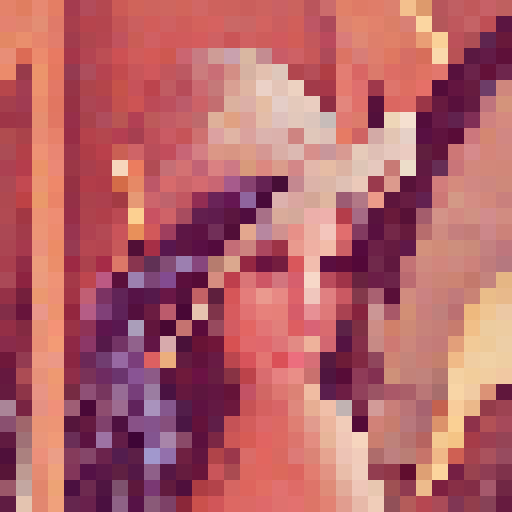
\includegraphics[width=0.1\textwidth]{dyadic_4.png}}%
\hspace{.2in}%
\subfloat[$C=128$]{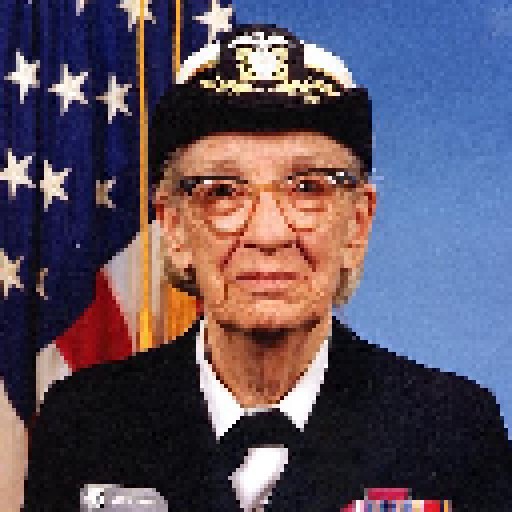
\includegraphics[width=0.1\textwidth]{dyadic_8.png}}%
\hspace{.2in}%
\subfloat[$C=512$ (Original Size)]{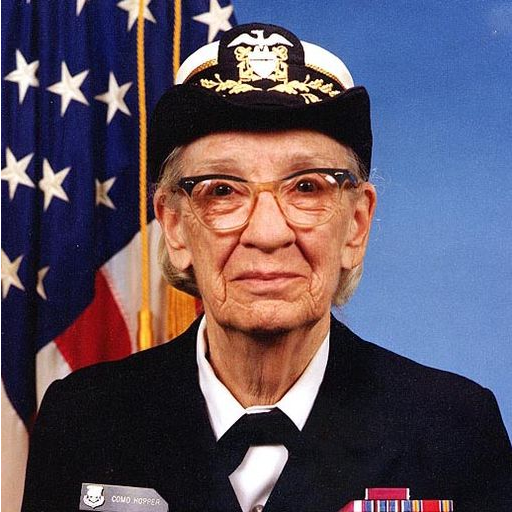
\includegraphics[width=0.1\textwidth]{dyadic_16.png}}%
\caption{Example of dyadic space using an image of Grace Hopper (512x512
pixels) at different dyadic scales ($C$), note how the picture becomes less
pixelated at higher scales}
\label{fig:dyadic-image}
\end{figure}

A natural interpretation of multifractal analysis needs to be based on wavelet
leaders, which allows an estimation of the multifractal spectrum of an image.
The wavelet coefficients at finer scales within a small neighbourhood are used
to renormalise the wavelet coefficients at a given scale.

This is all theoretically very sound, but in practise it cannot be used on
paintings without some modifications, mainly due to the fact that digital
objects do not have an infinite resolution. So the analysis is slightly
simplified to account for this to provide a fair estimation of the real
analysis.

This technique was applied to several different works, but the most interesting
of there was the Princeton experiment, where an artist produced seven distinct
small paintings using different materials. Two weeks later the artist was asked
to produce replicas as close to the original as possible.

Both the originals and replicas were scanned at a very high resolution to allow
this analysis to be as detailed as possible.

The results showed that, systematically, the textures of the replicas were
globally more regular and smoother than the originals. However, it should be
noted that getting these results required the expert selection of sections to
analyse and the a posteriori selection of the range of scales for wavelet
leaders.

With promising results shown from this experimentation, attention was turned to
a norm for painting analysis: van Gogh. Rather than consider the global state
of the canvas, each image was split into smaller sections for the analysis, as
paintings very rarely have the same texture globally.

This analysis was used to try and place paintings in a date region and detect
forgeries. The results shown for dating paintings into a period show some
promising results, where the majority of paintings were correctly clustered
into their correct periods. For detecting forgeries the results are promising,
but one forgery slips by when it was noticed by experts.

This technique is agnostic to the colour space and the authors do apply it to
several different colour spaces, including black-white intensity, \gls{RGB} and
\gls{HSL}.

There is a lot of expert knowledge which cannot be automated or, where it can
be, is very arbitrary such as blindly selecting patches.

The results from the Princeton experiments are promising, but the results are
very sensitive to the material of the canvas as well as the tools used, whilst
this might be use for detecting forgeries, there might be situations where this
isn't desired.

The images the authors use are high resolution (800 DPI) and they note that a
lower resolution makes it difficult to decide on the range of scales which are
involved.

The data sets used are relatively small and, although they increase the
knowledge by taking multiple patches from the van Gogh paintings, but for the
results they show only individual paintings are considered. One could easily
question the validity of their results based on this.


\subsection{Texton-Based Analysis}
% Paper 11

Analysis of texture can also be performed with the help of a set of small
patches, or textons, relating to the texture of the image. An interesting
approach is to learn a variety of these textons from example images and then
look at a histogram of the frequencies of these textons on the images to
classify\cite{van2010texton}.

Segmentation of brushstrokes is, understandably, difficult - especially
digitally where the image is usually only two dimensional, but one can consider
the texture of the painting with more ease and can provide a good insight into
the artists style.

Filters are becoming less popular for painting analysis as the filter often
normalises the image to a certain extent in the process of analysis. Other
approaches like wavelets and pixel-based representations, such as texton
approaches, are becoming more popular to avoid this issue.

It should be noted that whilst textons are a building block of the text of an
image, they are not identical to brushstrokes.

To construct the codebook of textons, 5000 patches are selected in random
locations from each painting in the training set. These patches are then
clustered and the most exemplary patch (the central patch) is selected as the
most representative for that cluster.

From this codebook it is then possible to generate a histogram for any image
which estimates the distribution of these textons across the image. The
histogram is created by applying a sliding window across the painting and
selecting the nearest texton in euclidean space to the window. Finally the
histogram is normalised to sum up to 1.

The authors note that these histograms could be built up for different sizes of
textons to increase the feature space available for analysis, for their own
experiments they use six different scales of texton.

Because the aim of this research was to work closely with experts in the field,
the authors also came up with a method for visualising this information. For an
image processing system this may not be required, but could be used to extract
more useful information from the analysis.

Because of the high dimension space it is necessary to reduce the
dimensionality of the results to allow it to be human readable. Usually this
would be performed by \gls{PCA}, but the way in which the data is structured,
\gls{PCA} is too lossy for texton histograms; it has a linear nature whist the
texton histograms may be high-dimensionally non-linear and it focuses on
preserving the global structure rather than local structure of high-dimensional
points.

There are other techniques which might have been applied to solve these
problems, but the authors found some shortcomings with these techniques which
would have made real-life visualisation difficult.

To cope with this, a new method for dimensionality reduction was invented:
\gls{t-SNE}. This method hinges around keeping
the conditional probabilities between the high and low dimension spaces
similar.

Interestingly, in the experiments \gls{PCA} was first use to reduce the
dimensions down to 50, and then \gls{t-SNE} was
used to reduce down to two dimensions. Suggesting that, for very high dimensions,
\gls{t-SNE} is not very effective.

The results on 117 high-resolution grayscale van Gogh paintings show that most
of the non-van Gogh paintings appear on the peripheries of the visualised
two-dimensional graph, apart from two specific forgeries: the Wacker forgery
which had fooled experts for many years, but can successfully be found by
looking at global features. The other, created by Gaugin, may remain undetected
for the same reason.

Visualisation of dated van Gogh work does show some difference between the two
time periods considered, but not enough to cluster or classify upon with any
degree of accuracy.

% How many clusters?

This approach is definitely a useful one, especially given that the textons are
learned from existing work, making analyses such as trying to date an artists
work from sets of his known work very applicable. Although colour and global
features are not considered by the textons described in this work, colour would
be a simplistic feature to add and global features could be part of a separate
technique which is later included with the histogram.

The paper does leave some answered question, one notable one is how best to
decide the number of clusters to build the texton histogram from and which
scales the textons work best at. For use by experts with \gls{t-SNE} applied
this might be some useful work, but \gls{t-SNE} seem to have limited
application outside this form of data set. A comparison between \gls{PCA} and
\gls{t-SNE} would, perhaps, show the advantage of the latter and an explanation
as to why \gls{PCA} was applied before \gls{t-SNE} on their own experimental
results would help others to better apply such methods correctly.

\section{Statistical Analysis}

A lot of analysis can be gained from passing filters over an image and
considering the colours used. However, a lot of these depend on some way of
statistically analysing the results. This section will look at some of the
research that considers some of the more statistical elements to provide
analysis.

Whilst gaining results of analysis techniques, it is also important to be able
to interpret them digitally for some form of use; determining whether a
painting is authentic or not, or dating an artist's work within a set of their
known work.

Often these techniques involve using a form of machine learning to gather
meaningful data from the high dimensional feature space which image processing
processes provide.

\subsection{Stylistic Analysis}
% Paper 9

All artists have a distinguishing style which may change as their career
progresses. Art historians find this a challenging problem as many factors of
the painting need to be taken into account. Image processing and machine
learning techniques can be used to aid this process.

Stylometry, the study of an artists style, has many problems involved with it.
Two of these are: extracting distinguishing features and dating a
painting, both these problems are tackled in \cite{jafarpour2009stylistic}.

This research uses considers the artists style to be a hidden variable which
controls the observable properties of the image; the colour, brushstrokes, etc.

The dating challenge is the act of dating a painting from a catalogue of known
paintings from the artists lifetime. An artists style is likely to change over
time, especially as they meet their peers and try out new movements.

This research considers how a human expert might approach the problem of
determining style and that paintings may degrade over time due to the materials
used to create them. Historians must combine a potentially noisy observation
with pre-existing knowledge to come up with an analysis of the style.

Computer systems have to use features of an image, considering both global and
local information, to build up a high-dimensional feature space which can then
have statistical analysis performed upon it to gauge some information about
style.

It has already been discussed that a \gls{HSL} colour space provides a more
representative view of an image than a \gls{RGB} space. However, \gls{HSL} does
not exist in a Cartesian space. This can be achieved by transforming the
\gls{HSL} space into an XYZ space by ``unrolling'' the radial elements of
\gls{HSL}.

As with many techniques which utilise wavelet transforms, a very high
resolution is used to gather information which may be too fine for a human eye
to perceive. A dual-tree complex wavelet transform using the aforementioned XYZ
colour space can detect colour patterns as well as local difference.

These wavelets provide coefficients in very high dimensional space which a
large amount of noise. To deal with this there is a need for dimensionality
reduction and normalisation of noise within the feature space.

Hidden Markov Trees provide an image model over numerous different resolutions.
They act like Hidden Markov Models but also considers a tree like structure
which maps to dyadic space. This allows for an image to be described as a
statistical entity rather than a set of pixels.

At each scale there are hidden variables which control the wavelet
coefficients. These hidden variable represent either a smooth region, which has
a small variance, or an edge, which has a large variance.

The images are split into several patches to allow the analysis to be performed
effectively.

Results for the dating challenge, 66 van Gogh paintings were used with the goal
of dating three test images which cannot be easily dated by art historians.
Training was performed on the set of paintings using 10-fold cross-validation
using several different classifiers. The best classifier; random forest; had a
generalisation performance of 73.7\% and the results from the three test images
aligned with the conclusions of the art historians, but this is somewhat
conjecture as the dates aren't officially known.

Extraction distinguishing features focused on extracting flowers within the
paintings. Irrelevant patches were removed from the training images and again
training was performed using 10-fold cross-validation using several
classifiers. Once again random forest was the best decision and several
distinct distinguishing features.

The results of this research do seem promising, and the techniques described
here do seem like they can provide some very powerful analysis.

The sample size is a little small, but the split into different patches allows
for a larger number of samples for training. Though this still only has a
certain number of date ranges to work with.

The size of the patches is never fully explored and the research blindly uses
$256 \times 256$ pixels for each region. It would be interesting to see what
effect changing the size of these regions would make upon the research.


\subsection{Authentication of Artwork}
% Paper 4

Another interesting problem within the field of art analysis is the problem of
many hands; that is determining how many authors created a work and which parts
of said work can be attributed to which author. Obviously, the latter can also
be simplified to test which artist created a work and thus detecting forgeries.

One attempt to attempt to solve the many hands problem is described in
\cite{lyu2004digital}. As with much of the recent work into applying image
processing to artwork, it considers paintings at multiple resolutions and
orientations using wavelets.

The method for this technique is to decompose the image using wavelets. In this
paper quadrature mirror filters; filters which split an input signal into two
bands; are used to split the frequency space into multiple scales and
orientations. This produces a statistical model at each scale and orientation;
known as a subband.

The optimally predictive set of neighbours is selecting by minimising the
prediction error using a brute force iterative approach on a per-subband and
per-image basis across all subbands.

Additional statistics are also gathered from the errors of the final predictor,
again for each subband. For $n$ levels of decomposition, this will produces
$24(n-2)$ values ($12(n-2)$ for optimal predictors, $12(n-2)$ for error
statistics).

These large dimensional spaces can be projected into a human-friendly subspace
using a process named \gls{MDS}. \Gls{MDS} attempts to maintain the distance
between data points when projecting into a lower dimensional space so should
still provide a decent visualisation of the higher dimensional space.

The first experiment focused on authenticating the work of Pieter Brugel the
Elder who used very distinct style which the authors felt would be especially
applicable to their technique. A set of 13 paintings conprising of 8 authentic
Brugels and 5 famous imitations was the subject for this analysis.

Each painting was scanned in very high resolution and was separated into 64
non-overlapping regions. Each subimage was transformed the proposed wavelet
transform at five levels and three orientations producing a 72 dimensional
space. Authentication was performed by applying Hausdorff distance to this
space with the assumption that authentic paintings would be closer together.

This these experimental results it did indeed show that this was the case and
are statistically significant, even in a reduced feature space through
dimensionality reduction.

This was also to applied to a painting by Pietro di Cristoforo vannucci
(Perugino) which is disputed by art historians to have been produced by more
than a single artists, which, during the Renaissance was common amoungst the
great works.

This effect is commonly observed in the six faces which are depicted in this
painting. These faces were first selected and then partitioned into $256 \times
256$ regions as with the Brugel work. The technique was then applied and
Hausdorff distance was measured between the feature spaces. Viewing the results
shows an obvious clustering of three of the faces, whilst the other three are
completely separate from this cluster and from each other. This would suggest
that there were at least four hands involved in the painting, which is
consistent of the views of some art historians.

The sample size both experiments were performed on is relatively tiny when
compared to other studies using similar techniques. One could easily question
the validity of such results, especially with the subjectivity of the second
experiment where there is no definitive answer.

The work of Brugel is noted to have delicate lines and shading which was
expected and shown to have good results. A cynical reader might infer that this
analysis technique is therefore not suited to other styles of art.

It's also interesting that the Brugel paintings were cropped to a given size
before being split into regions as this would surely lead to loss of
information when it might have been better to just increase the number of
regions across the image to include the whole image.

As with other research including wavelets the dependence on a region size of
$256 \times 256$ pixels is notable. This appears to be a standardised size for
the application of wavelets, but there appears to be no documentation of this.

% Line shaded -> applicable to paint?
% Crop size -> loss of information

\subsection{Dating an Artist's Work}
% Paper AWESOME :D

Another avenue which can be taken is to use an artist's existing work to try
and classify new examples. \cite{brown13can} describes one attempt to do this
using a variety of techniques, from colour analysis to texture details.

To verify the results gained from this research the authors used a
leave-one-out cross-validation strategy on the 102 works for which a date was
know. This provided a correlation between actual year and classified year, as
well as the statistical significance of these results and the number of
paintings which were successfully classified within 15 years.

Analysis techniques provided results in the form of histograms which could then
be used to measure the distance between an example and the training set and
classified using $k$-nearest neighbour. This classification algorithm was used
because of its simplicity and naivety, which allowed it to only consider
distance in the feature space rather than any patterns in the underlying data.

Graphing the results of the classification a ``best'' value of $k = 7$ for
$k$-nearest neighbour was selected visually and used to gather formal results.
These results show correlations approaching $0.5$ for some of the more advanced
techniques; those examining the texture of the work.

This research also considered the idea of exemplar paintings; those paintings
which are most representative for a given year. Expert knowledge was used to
produce a list of \emph{Artistic Exemplars}, those most representative of the
artists style to an expert in the field. From analysis of a group of paintings
for each year a central point was computed, then the closest painting to this
central point was chosen as a \emph{Statistical Exemplar} for that year.

These exemplars were then used to classify other paintings by labelling the
painting with the nearest exemplar. Though these don't show as good correlation
results, it does allow other avenues of work to be created such as
investigating the differences between the \emph{Artistic} and
\emph{Statistical} exemplars.

This work does start tcentral point was computed, then the closest painting to
this central point was chosen as a \emph{Statistical Exemplar} for that year.

These exemplars were then used to classify other paintings by labelling the
painting with the nearest exemplar. Though these don't show as good correlation
results, it does allow other avenues of work to be created such as
investigating the differences between the \emph{Artistic} and
\emph{Statistical} exemplars.

This work is obviously in its infancy but does show some promising results. The
methodology is well thought through.

The authors do discuss the use of $k$-nearest neighbour and whether it should
be compared to other classifiers. An \gls{SVM} seems particularly applicable as
it would help draw out some of the underlying patterns in the artists work.

The lack of high-resolution images with non-standard lighting has hindered this
research somewhat; although part of the point of the research is that the
system should be robust enough to handle simple catalogue images, it does
appear to damage the performance.

It is also very specific to the artist Kyffin Williams, as his work was highly
textural, which might explain why features including texture performed better.
More work could be done to explore other artists and see how they compare to
Williams.

As the work uses histograms, it might have provided better results to combine
the results of the analysis techniques to gather a larger histogram. This would
have to be normalised or weighted based on the performance of the techniques to
gather meaningful analysis, but is another avenue which hasn't been explored
sufficiently.

\section{Brushstroke Analysis}

The ideal technique for analysing a painting digitally is to be able to extract
brushstrokes from the painting and be able to analyse them based on their
shape, colour and where on the painting different types of stroke were made.

This is a very difficult task, it may be easy for a human non-expert to view a
painting and roughly estimate where the surface brushstrokes are, implying that
an expert may be able to tell far more from a detailed view of the painting,
including multispectral imaging using X-rays.

For a computer to do this is a very intensive and complex task. As discussed
in section~\ref{sec:texture} is can be easy to view the texture of an image and
even to be able to pull out some information about the texture of brushstrokes.
But actually segmenting these brushstrokes for extraction quickly is a
different story.

This section will look into some of the research which has been attempting to
extract brushstrokes from paintings for the purposes of identification and
authentication of artwork. However, because this field is relatively narrow,
some exploration into extraction of brushstrokes in calligraphy will also be
considered as the fields have some overlap.

\subsection{Artistic Identification}
% Paper 1

To be able to extract brushstrokes it is important to understand how an expert
might go about the task. A lot of analysis techniques tend to be inspired from
how a human might go about the task, this also help a human to understand how
the process was gone about and may give extra meaning to the results.

There is a lot of knowledge to be gained from looking at the expert process,
and this knowledge can be applied to reduce noise and parameters from the
extraction process. The knowledge of painting materials, the state of the
preservation of the painting and the working methods of the artist themselves.

Interestingly, this leads to the conclusion that parts of the painting should
actually be discounted from the analysis, elements which have deteriorated over
time due to instabilities in the painting materials or the lack of preservation
of the painting leads to what most computer vision researchers would call
``noise''. Certain areas of the painting may not have been painting by the
artist's hand, such as cracks in the painting from the drying process, need to
be considered here.

It seems that it should be far more important to look at the areas where
brushstrokes were obviously painting ``rhythmically'': a series of fast strokes
arranged in a certain pattern, which can then be used to build up a personal
handwriting for a given artist\cite{johnson08image}.

Three different two-dimesnional wavelet transformation techniques were used in
this research:

\begin{itemize}
\item Penn State
\item Princeton
\item Maatrich
\end{itemize}

Penn State is an orthonormal series generated by a wavelet, implemented using
fast subband filtering, critically sampling the data.

Princeton forgoes critical sampling in favour of greater orientations using
complex wavelets.

Maatrich uses Gabor wavelets to provide a similar range of orientation
selectivity as Princeton, but in a way which is closer to a physiological
templates.

Because of the differences between these wavelet transforms, different
classifiers need to be applied to the resulting coefficients.

Both Penn State and Princeton transforms can use a hidden Markov model
approach. Because Markov models have states which are linked to the predecessor
or neighbour states with a probability distribution. Hidden Markov models are
Markov models where this probability distribution is unknown and can be
inferred from the data which constructs the model.

There are several classifiers which can be applied to Markov models, although
typically these relate to some form of expectation maximisation technique.

All experimental results were gathered from a data set containing 101 paintings
in the style of van Gogh. 82 of which are believed to be true van Gogh works,
13 which are currently in dispute and 6 which are known imitations. All of
these paintings are scaled using the same technique to be equivalent sizes.

The approach for using Penn State was to gather several unquestionably van Gogh
paintings which are representative of his style (exemplar images) as a training
set. By not including negative examples in the training set the resulting
classifier is more stringent.

The paintings are then divided into patches of roughly $512 \times 512$ pixels
such that all the patches from the same painting are the same size.
Dissimilarity measures between these patches are calculated using both texture-
and stroke-based features. Paintings are then compared using the aggregated
distances between the patches of the images.

Texture features were extracted in a form which shows the abruptness of changes
in variations at different orientations. Textures were only captured at the
highest scale. These are then put into a feature vector which can be converted
into a Markov model.

For extraction of strokes an edge-detection algorithm is used to detect
contours of the image, which can then have several geometric features computed,
such length, average curvature and orientation.

Because textures are dependent on their neighbours it is sensible to build up a
probabilistic model, namely a Markov model, to show these dependencies. Because
the probabilities which affect the dependencies are unknown this must therefore
be a hidden Markov model, using two dimension (as images are two-dimensional).
A likelihood classifier can then be trained from the training set and applied
to other 2D hidden Markov models to be able to classify examples.

Spatial features are less important for brushstrokes as they capture more
global information rather than information which is likely to be affected by
neighbouring strokes. Clustering can be applied to this to partition the data
set then new examples can be classified using the distances to these clusters.

Princeton shows the scale at which details start to emerge; each patch is
analysed using the wavelet transform and then these coefficients are stored is
a hidden Markov tree in a similar process to \cite{jafarpour2009stylistic},
where the hidden states take the form of edge or non-edge. This helps show the
scale at which an individual artist's style emerges as the transitions between
edge and non-edge will occur at different scales.

Only 79 of all 101 paintings were analysed by Princeton, the other paintings
were too dark for meaningful analysis to be gained from them in this
experiment. 65 of these were van Goghs, 6 imitations and 5 of the questioned
paintings.

\gls{MDS} is used to find an arrangement of all the points in a three
dimensional space (as opposed to the very high dimensional space the hidden
Markov tree uses. For all van Gogh paintings the centre point is determined,
where all of these paintings are equally weighted.

The 3D visualisation shows a good separation of the van Goghs from the non-van
Goghs, but to be able to truly use this, a radius classifier is applied such
that a lower radius is more likely to classify as a van Gogh and visa versa. An
appropriate point $r$ is chosen as the cut distance at which the label changes,
such at van Gogh paintings are closer to the centre than $r$.

This classifier was tested using leave-one-out cross validation; a validation
technique based on $k$-fold cross validation where $k$ is the size of the data
set. $k$-fold cross validation partitions the data set into $k$ subsets. Each
subset has classification performed on its elements based on training from the
other subsets.

Leave-one-out cross validation is a useful cross-validation technique for small
data sets and can be used to gather a correlation of expected output against
classified result. This can also be used to gather the statistical significance
of the results.

Biologically inspired techniques have shown promising in other fields of
computer science, notably items like Artificial Neural Networks, Immune and
Endocrine Systems; Swarm Intelligence such as Ant Colony Optimisation; etc.

Using the human visual system as a metaphor paintings can be analysed using
three principals:
\begin{inparaenum}[1)]
\item Importance of contours;
\item Analysis at multiple scales;
\item Similarities are reflected in local textures.
\end{inparaenum}

The Maatrich transform uses Gabor wavelet filters at multiple scales and
orientations. The provides an ``energy'' value for each pixel, orientation and
scale. These values can then be binned into a high-dimensional histogram. This
allows a \gls{SVM} to be trained and new example to be classified
with. Because there are only two states (van Gogh and non-van Gogh), a
\gls{SVM} is a good classifier. Again, leave-one-out cross-validation is used
for each painting, the patches are separately classified then the most
frequently returned label is used to classify the painting.

% PS results
Penn State begins to show some good results, although one of the imitations is
considered to be one of the five closest to the training set of 23 van Goghs.

% Pr results
The radius classifier applied to the Princeton tranformation successfully
classified 55 of 65 van Goghs and 9 out of 11 non-van Goghs correctly. At even
finer scale shows even better results.

% MA results
Maatrich transforms with a \gls{SVM} classifier successfully classified four of
the six non-van Goghs correctly, but wrongly classifying two of the van Goghs.
This starts to show that it can detect dissimilarities in the brushstroke
texture of a painting, but that some difference may be too subtle to pick up.

% Conclusions
The use of leave-one-out cross-validation means the experimental results are
very valid; but the lack of significance does remove some of this validity - it
is up for debate whether a null hypothesis could also be to play.

The images are high resolution greyscale, so although colour information has
been lost but the resolution means that most of the paintings should be uniform
and detailed.

The discussion and use of expert knowledge means that the results gained are
potentially more valid by not considering several sections of a painting.
However, the opposite argument could be made that part of van Goghs style was
to deform the paintings slight by leaning against them, etc. and therefore is a
better indicator of his style than some of the brushstrokes.

This does show positive results and the techniques are well thought out,
including discussions of other classifiers which could have been used.

As is a common problem in brushstroke extraction there is no ground truth on
which these techniques can be applied to, so it is difficult to know how well
these techniques will apply to other paintings by van Gogh or by different
artists.


\subsection{Rhythmic Brushstrokes}
% Paper 2

Using computer vision to segment brushstrokes is a difficult task; often
requiring expert knowledge of the painter and manual intervention to enable the
process. \cite{jia12rhythmic} shows a method for the automatic extraction of
brushstrokes.

This method involves a complex process; first the image has an edge detection
algorithm applied to it, then these edges are pruned to remove noisy, short and
unconnected edges to improve the actual segmentation of strokes.

Because an edge detector doesn't always pick up the full brushstroke, any gaps
in the painting are enclosed using a greedy process of scanning neighbours and
linking the nearest via a straight line if they are within a certain distance.

Any fully enclosed brushstrokes are then extracted and checked against an upper
and lower threshold for size. These thresholds were pre-selected to give a good
estimate for the size of a brushstroke. This is finally labelled a brushstroke
if the backbone is not too branched, it has a reasonable ratio of broadness to
length and the size of the stroke is proportional to the backbone of the
stroke.

After this process is complete, the image is then segmented with regard to
colour (\gls{RGB}) and directions (horizontal and vertical). $k$-means
clustering is then applied multiple times, gradually decreasing the threshold
for the average distance in the cluster. Any sufficiently small clusters are
removed at each step and are not considered in the future runs of the $k$-means
algorithm. This process is done to remove any noisy components there might be
in the digitisation of the image.

Brushstrokes which are already labelled are then removed and any remaining
clusters are labelled according to the same process.

Calculating the backbone is based on the edge detection of a segmented
brushstroke, this will generally form ``Y'' shaped structures; in the case of a
few of these structures, the shortest branch is simply removed. This process
might produce a disconnected backbone, at which point it is labelled
``severally branched''.

To gain experimental results, 45 digitised oil paintings from van Gogh and his
contemporaries were used, ranging in sizes and scales. A ground truth for the
brushstroke extraction was generated manually from 10 regions of these
paintings.

First, the system used to decide if a region is a brushstroke was evaluated on
these manually generated brushstrokes, obtaining a correct decision 95\% of the
time.

Then, the automatically extracted brushstrokes were compared to the manually
selected ones in terms of: validity (the percentage of extracted brushstrokes
which are in the ground truth) and detection (the percentage of the ground
truth strokes which were extracted).

Validity reached an average of 60\%, but ranged between 42\% and 83\% for
different paintings. Detection also reached and average of 60\%, but the lowest
was 22\% and only reached a high of 75\%.

Of course, the extracted brushstrokes also need analysis performed on them.
This is where the backbone calculation can also be used to extract features out
of the brushstroke, as well as considering the features of the brushstroke
itself.

Using this statistically, this can be used to authenticate paintings and also
begin to place them in different periods. However, the results from these are
in terms of $p$-values for each feature and do not consider multiple features.
However, it was found that the features which distinguish van Gogh from his
contemporaries are not the same as the ones which differentiate two different
periods in van Gogh's career.

These results are very promising, especially given that the brushstrokes were
compared to a ground truth. Of course it could be argued that the ten regions
selected were done so to show the best of the technique, but given the
visualisation of the brushstrokes, this seems unlikely.

It would have been interesting research to see how the threshold values for the
detection of a brushstroke; there is no investigation or discussion as to why
the high and low values were set where they were.

The same goes for $k$-means clustering; is there a better choice which provides
more accurate clusters, and therefore strokes, or was it chosen because of its
simplicity and the benefits gained from using a more complex one wouldn't be
worth the computational complexity?

One would have thought that a density-based clustering algorithm such as
DBSCAN\cite{kriegel11density} would have been more applicable to this problem
as it would have been able to cope with noise and may have provided a better
segment of the brushstrokes.

There is also the question of applicability. That is, this has been 
successfully applied to van Gogh and some of his contemporaries with oil
paintings, but would the technique still yield such good results is applied to
an artist who used a palette knife, etc.?


\subsection{Stroke Decomposition}
% Paper 15

One interesting use of stroke extraction is to animate Chinese paintings from
an original\cite{xu2006animating}. This is a complex procedure which involves
decomposing the painting based on brushstrokes, these brushstrokes can be
represented as vectorised elements and become easy to manipulate and therefore
animate.

To decompose the strokes the following method is proposed.

First, the image is over-segmented using a mean-shift algorithm, this is done
because colour is required to extract brushstrokes, but is not enough alone.
The over-segmentation stops regions spanning across multiple strokes, unless
the strokes themselves are overlapping.

The strokes are then extracted by merging these regions until they represent
the brushstroke. This requires some domain knowledge as naively merging these
regions may not represent the stroke accurately enough.

Two intuitions are used in this research: colour gradients are low along brush
strokes and strokes will match a library of strokes manually extracted from
other sources. 

To merge the segmented regions a region merging criterion $\epsilon$ is
calculated. $\epsilon$ is then used to merge adjacent regions from highest to
lowest. $\epsilon$ is calculated in terms of the differences in colour
distribution between the regions and the similarity to the catalogue of
brushstrokes.

Once this process is complete, the strokes can then be refined and vectorised
for the animation process.

This paper also considers the separation of overlapping strokes to be able to
animate them naturally, but this could potentially be used for further
analysis. The overlapping regions can be identified in the segmentation process
then have an iterative algorithm which separates the colours of the overlapping
region. Because the colouring of an overlapping region can be the mixture of
more than a single colour, a mixture model is used to model the overlapping
strokes.

Combining this with the library of known strokes can be used to get a good
estimate of the separate strokes.

This paper presents some really interesting research into the decomposition of
paintings using brushstroke extraction; but is very specific to Chinese
paintings. An example failure run on a painting by Georges Seurat shows the
overfitting which this method falls prey to.

The reliance of a catalogue of brushstrokes seems to do more harm than good in
some circumstances, the authors do note that the catalogue is by no means
exhaustive. This is what seems to lead to the over segmentation. Perhaps
learning the strokes from existing work as discussed in \cite{van2010texton}
could provide more generalised results.

Unlike \cite{jia12rhythmic}, the extracted strokes are not evaluated against a
ground truth. Even so, the visualisation of the segmented brush strokes seems
reasonable and to be able to complete the animation steps there must be some
validity to the extraction process.

The development of a technique to discriminate two overlapping strokes shows
some potential, although there is no real verification of the method to do
some. It should also be noted that the paper only considers two overlapping
strokes as more would become too computationally complex to complete in a
reasonable time. 

\subsection{Calligraphy Stroke Extraction}
% Paper 14

Chinese calligraphy is a painted art in its own right, although not exactly
like a painted scene it does provide some insight into stroke extraction which
has a much more formalised ground truth.

\cite{xu2005automatic} described a method for the automatic extraction of
calligraphy strokes, with account for differing stroke sizes, deformations and
noise found in historical work.

Unlike paintings, Chinese calligraphy is only comprised of a certain catalogue
of strokes and are categorised into either basic or composed strokes.

The input, a binary image, has the Canny edge detection
algorithm\cite{canny86computational} performed on it to extract the edge of the
character.

Because calligraphy strokes often overlap, the corner points of the edges of
the character are found preserving information about the direction this process
was performed in.

A half-edge colouring graph can be created to show the relations between
different edges. Each edge is split into two half-edges which has colours
according to the relation to other edges. This information, plus the direction
information allows the computation of matching different edges to build a
single stroke, with relation to the distances of different vertices.

This is done by removing the largest edge then trying to find one or more edges
which can match to it to make a stroke. Once the stroke is found it can then
have the gaps filled in by linking the two nearest vertices.

There is little experimentation and no formal validation performed other than a
visual check. The authors even note an occurrence where the corner detection
algorithm failed to provide reasonable vertices and so the strokes had to be
extracted manually.

One would have though in an area where it would be easy to generate a ground
truth, it would have been used to at least perform some form of statistical
analysis on the results gained.

This might be useful in edge cases of digitally analysing paintings, but
without knowing how well it truly performs on calligraphy, one might be
hesitant to apply this to a what is a much more complex field which needs the
consideration of colour as opposed to a binary intensity.

Whilst there are claims this technique should be able to cope with noise from
historical degradation of the image, it is difficult to see how. Especially as
Canny is known to susceptible to noise and can be improved to be less
sensitive\cite{xiao10improved}.

\section{Conclusions and Summary}
% TODO beast mode this.

Digital analysis of artwork is not a trivial task: there are many problems
which occur far more prevalently than in other fields of image processing. The
need for high-resolution copies of artwork with a standard method of capture
can significantly hinder some areas due to the lack of availability.

Added to that, noise is far more common from degradation of works from a lack
of care or poor materials used to create the piece. Although this is a
two-sided coin and there are analysis which could be performed which look at
specific types of degradation to authenticate an artwork.

With all the different kinds of art and materials which can be used to produce
works, it is very difficult not to over specialise in the analysis techniques,
especially when it comes to complex techniques such as detecting brushstrokes.

Texture appears the be the base of a decent analysis technique; most of the
brushstroke extraction technique use some form of texture discrimination to
function. Colour does provide some interesting results, but it is usually the
cumulation of texture and colour which provides the most powerful analysis.


% conference papers do not normally have an appendix


% use section* for acknowledgement

% trigger a \newpage just before the given reference
% number - used to balance the columns on the last page
% adjust value as needed - may need to be readjusted if
% the document is modified later
\IEEEtriggeratref{17}
% The "triggered" command can be changed if desired:
%\IEEEtriggercmd{\enlargethispage{-5in}}

% references section

% can use a bibliography generated by BibTeX as a .bbl file
% BibTeX documentation can be easily obtained at:
% http://www.ctan.org/tex-archive/biblio/bibtex/contrib/doc/
% The IEEEtran BibTeX style support page is at:
% http://www.michaelshell.org/tex/ieeetran/bibtex/
\bibliographystyle{IEEEtran}
% argument is your BibTeX string definitions and bibliography database(s)
\bibliography{bibliography}

% that's all folks
\end{document}
